\subsection{Allgemeines}

Bevor man sich mit dem Design und der Implementierung einer Serverless Infrastructure Anwendung beschäftigen kann, ist es notwendig sowohl Begriffe wie Cloud Computing und Serverless zu erklären als auch alle wichtigen Cloud Computing-Modelle darzustellen und miteinander zu vergleichen.

Das Modell Function as a Service ist eine logische Fortführung der bisher existierenden Servicemodelle.
Somit sind auch diese Grundvoraussetzung für das Thema Serverless.
Im folgenden Abschnitt werden all diese erforderlichen Voraussetzungen geschaffen und die einzelnen Cloud Computing-Modelle miteinander verglichen.


\subsection{Definition und Erläuterung}
Der Begriff Cloud Computing beschreibt im Wesentlichen die Bereitstellung von Ressourcen über das Internet.
Hierbei kann es sich um jede Art von Ressourcen handeln. Dazu zählt zum Beispiel die Netzwerkinfrastruktur, Server, Speicher, Datenbanken aber auch Software.
Anwender zahlen nur die tatsächlich genutzte Leistung und können den Bedarf jederzeit flexibel anpassen.
Lokal muss in der Regel nur ein geeigneter Client installiert sein, etwa ein Webbrowser.

Die wichtigsten Vorteile gegenüber einer On Premises-Landschaft sind die schnelle Verfügbarkeit und Skalierung von Diensten, sowie dass keine Kosten im Voraus entstehen.
Durch den Einsatz von Cloudtechnologien verlagert sich das Kostenmodel von Capex\footnote{ Capex(Capital Expenditure) bezeichnet Investitionen und Ausgaben die einmalig getätigt werden,
um den Umsatz zu erhöhen. Dazu gehört zum Beispiel die Anschaffung von neuer Hardware. } zu Opex\footnote{Opex(Operational Expenditure) bezeichnet wiederkehrende Kosten wie Verwaltungs- und Betriebskosten.
Auch fallen mittlerweile viele Softwarelizenzen regelmäßig an. }.
Mit einem Knopfdruck ist es möglich beliebig\footnote{Das Wort beliebig ist nicht sinngemäß zu verstehen.
Auch Cloud Provider haben nur eine endliche Anzahl von Kapazitäten und geben den Kunden diese nicht in vollem Ausmaß frei.
Jede Umgebung eines Kunden hat bestimmte Limitierungen pro Service, die jedoch bei Bedarf eventuell angepasst werden können.
AWS erlaubt beispielsweise pro Region und Account 2880 vCPUs für Standardinstanzen } viele Ressourcen und Dienste hochzufahren und zu verwenden.
Je nach Servicemodell verschiebt sich der Verantwortlichkeitsbereich zwischen dem Cloud Provider und dem Anwender.
\cite[]{CloudComputingDef}

\clearpage

\subsection{Cloud Computing-Modelle}
\label{Servicemodelle}
Zur Veranschaulichung der unterschiedlichen Servicemodelle dient folgende Grafik.
Im Anschluss werden die einzelnen Modelle im Detail beschrieben.


\begin{figure}[htbp]
    \centering
    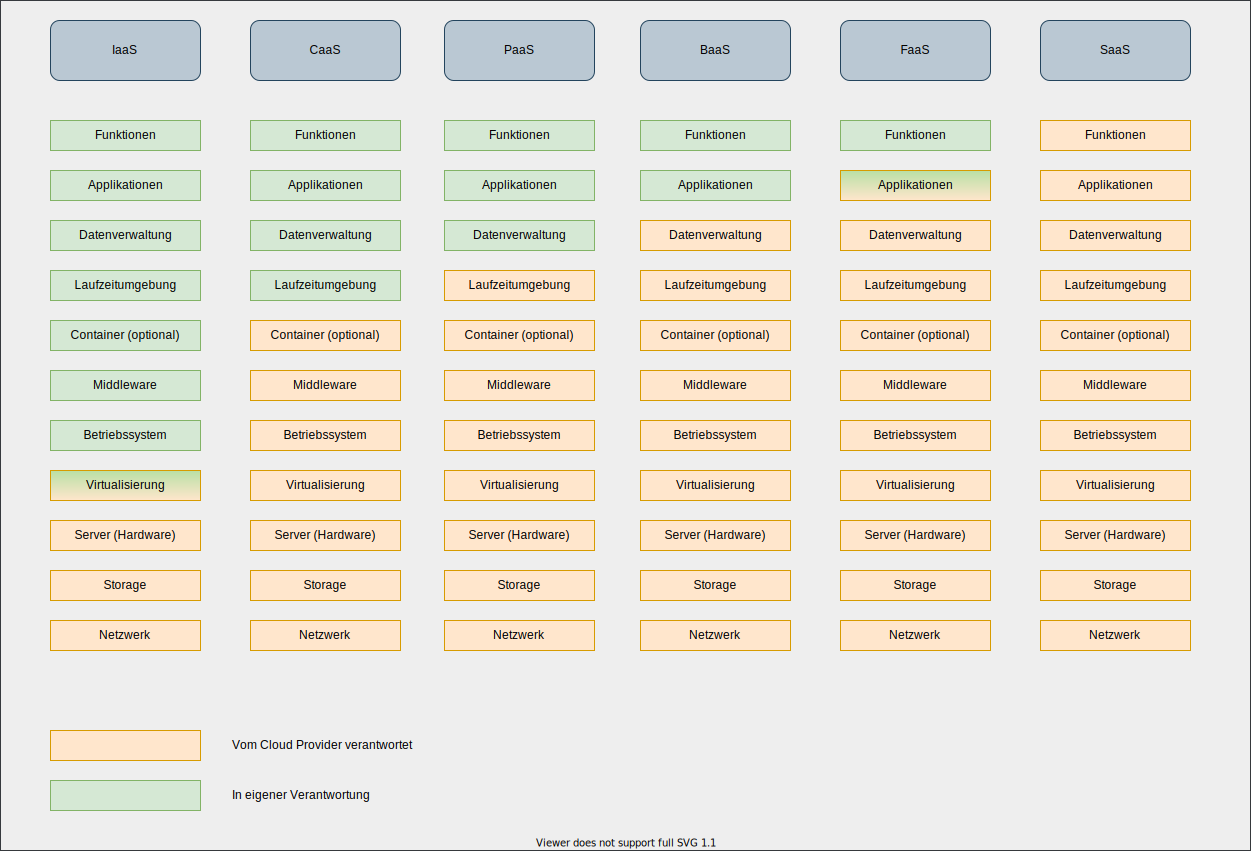
\includegraphics[width=1.0\textwidth]{30-Serverless-Theorie/ServiceModelle.png}
    \caption{Übersicht der Servicemodelle}
    \label{fig:meine-grafik}
\end{figure}


   \subsubsection{IaaS: Infrastructure as a Service}
   Unter dem Begriff Infrastructure as a Service, kurz IaaS, versteht man Infrastruktur bei der Administratoren bzw. Anwender sowohl die größte Kontrolle als auch die höchste Verantwortung tragen.
   Der Cloud Provider kümmert sich nur um die nötige Infrastruktur um Computing-Ressourcen über das Internet zur Verfügung stellen zu können.
   Dazu gehört der Erwerb und Betrieb von Servern, Switchen, Routern und Speichersystemen und der Virtualisierung von Maschinen.(siehe Abbildung \textit{\nameref{Servicemodelle}}).
   Dieses Modell ist am ehesten mit einer On Premises Infrastruktur vergleichbar und bietet eine hohe Vertrautheit und Ähnlichkeit zu diesen Systemen.
   Im direkten Vergleich muss man bei einer Cloud-Lösung, irrelevant welches Servicemodell, kein Investitionsrisiko eingehen.
   Ist man sich unsicher über die benötigte Rechenleistung oder schwankt diese häufig kann, man jederzeit Ressourcen terminieren und Geld sparen.

   Das Betriebssystem inklusive aller damit verbunden Updates, die Regelung aller Zugriffe sowie die Installation und Wartung von Software liegen im Verantwortungsbereich des Kunden.
   Dieses Modell wird häufig verwendet, wenn man eine Hybridlösung mit einer On Premises Landschaft aufbauen möchte oder die eigene Applikation noch nicht für die Anwendung in der Cloud optimiert wurde, man diese aber trotzdem in die Cloud migrieren möchte.\cite[]{CloudComputingDef}

   \subsubsection{CaaS: Container as a Service}
   Container as a Service bezeichnet das Bereitstellen sämtlicher Ressourcen zur Verwaltung von Containern und der dort installierten Software.
   Unter Container versteht man ein {}\glqq Standardsoftwarepaket\grqq{} welches {}\glqq den Code einer Anwendung zusammen mit den zugehörigen Konfigurationsdateien,
   Bibliotheken und den für die Ausführung der Anwendung erforderlichen Abhängigkeiten\grqq{} bündelt. \cite[]{CaaS}
   Dieser gebündelte Container ist leicht portierbar und die Ausführung erfolgt in einer konsistenten Umgebung.

   Der bekannteste Dienst, um solche Pakete bereitzustellen, Docker unterstützt Windows und Linuxsysteme, sowohl OnPremises als auch in der Cloud.

   Das zugrunde liegende Betriebssystem und die Hardware werden für den Container abstrahiert.
   Dies führt zu einer kürzen Entwicklungszeit, da jeder Container reproduzierbar ist, und nicht individuell an das Betriebssystem angepasst werden muss.
   Auch können mehrere Container dasselbe Host Betriebssystem nutzen und sind dadurch schlanker und schneller einsatzbereit als klassische virtuelle Maschinen.
   Außerdem erleichtert es das Management von Patches sowie die Sicherstellung der Hochverfügbarkeit.
   Die Skalierung der Container kann der Cloud Provider übernehmen. Auch die Images lassen sich dort hosten und automatisiert deployen.
   In der Regel kommt Docker Swarm oder das ursprünglich von Google entwickelte Kubernetes zum Einsatz.
   Mittlerweile ist Kubernetes Open Source und wird von der Cloud Native Computing Foundation weiterentwickelt.

   Typischerweise werden Container as a Service zur Bereitstellung von Microservices verwendet.
   Das Container as a Service Angebot des Cloud Providers AWS heißt ECS (Elastic Container Service).
   AWS bietet Nutzern die Möglichkeit ihre Container entweder Serverless oder auf EC2-Instanzen\footnote{Amazon Elastic Compute Cloud-Instances(EC2) ist ein AWS Service
   zur Bereitstellung von virtuellen Maschinen in der Cloud. Es gibt viele verschiedene Instanztypen für jede Art von Anforderung.
   Zum Beispiel bietet AWS CPU, GPU oder RAM optimierte Instanzen in unterschiedlichen Größen an. } zu hosten. \cite[]{AWSECS}

   \subsubsection{PaaS: Plattform as a Service}
   Wie man bereits der Abbildung entnehmen kann, werden bei dem Servicemodell Plattform as a Service auch die Bereiche um die
   Containerbereitstellung sowie die Laufzeitumgebung von dem jeweiligen Cloud Provider übernommen. Für Kunden bzw. Anwender dieses Modells
   entfällt somit die gesamte Verwaltung der zugrunde liegenden Infrastruktur. Im Fokus liegt das Bereitstellen einer Plattform, die das
   schnelle und kostengünstige Entwickeln von Anwendungen ermöglicht.


   Anders als bei den vorherigen Modellen besteht hier keine Möglichkeit auf das Betriebssystem oder die Middleware zuzugreifen.
   Der Dienst muss mittels einer API oder einer Weboberfläche angesprochen werden.
   Dem Kunden werden zusätzliche Optionen zur Verfügung gestellt um leichter Testumgebungen erstellen zu können.
   Auch gibt es hier bereits vorinstallierte Dienste für Monitoring oder auch Alarme.
   Als Beispiele lassen sich hier etwa GitHub, Google App Engine oder AWS Elastic Beanstalk nennen.


   Elastic Beanstalk ist ein Service zum Bereitstellen von Webanwendungen. Da der Cloud Provider deutlich mehr Aufgaben übernimmt, kann der Kunde
   auch zum Beispiel nicht mehr alle Programmiersprachen verwenden, sondern muss sich auf eine von Amazon unterstützte festlegen.
   Im Gegensatz dazu muss nur noch der Quellcode hochgeladen werden und die Anwendung könnte auf Wunsch bereits im Internet erreichbar sein, ohne sich mit Themen
   wie Skalierbarkeit, Hochverfügbarkeit beschäftigen zu müssen. Für komplexere Aufgaben oder spezielle Anforderungen ist der Dienst eventuell weniger geeignet.
   Direkte Änderungen am System, wie eine Anpassung des Logverhaltens von Nginx, ist nicht möglich.
   Dafür bietet der Dienst Nutzern einen besonders leichten Start in die Entwicklung.

   GitHub ist ein Web-basierter Dienst, der öffentlich im Internet erreichbar ist, und Git für die Versionsverwaltung bereitstellt sowie weitere Funktionen zugänglich macht.
   Github wurde 2008 gegründet und 2018 von Microsoft aufgekauft. Auf dieser Plattform kann jede Person ihren Code(bzw. Dateien) veröffentlichen und teilen.
   Jeder Benutzer hat die Möglichkeit jedes andere öffentliche Repository zu klonen und selbst daran zu arbeiten oder auch dem Besitzer eines Repositories
   Anpassungen an den Code anzubieten. GitHub bietet viele Integrationen zu Cloud Providern an. So ist es möglich eine CI/CD\footnote{CI/CD steht für
   Continuous Integration, Continuous Delivery und Continuous Deployment und beschreibt eine Brücke zwischen Integrität von Daten und Automatisierung von Prozessen.
   Mit Continuous Integration wird, durch Zusammenführen und Testen, stets die Integrität des Quellcodes geprüft.
   Durch Continuous Deployment kann ein Softwarepaket automatisch in beliebige Umgebungen deployed werden. } Pipeline aufzubauen um voll automatisiert Ressourcen in der Cloud hochfahren zu können. \cite[]{GitHub}


   \subsubsection{BaaS: Backend as a Service}
   Dieses Servicemodell beinhaltet alle benötigten Dienste, um ein Backend für Entwickler zur Verfügung zu stellen.
   Entwicklern wird zum Beispiel ein Endpunkt bereitgestellt um Funktionen wie Push-Benachrichtigungen oder eine Social Media Integration verwenden zu können.
   Auch wird eine Datenspeicherung in relationale oder nicht relationale Datenbanken sowie das Hosting von Websites angeboten. Insgesamt gibt es einige Überschneidungen zu den anderen Servicemodellen.
   Backend as a Service wird genau wie Function as a Service als Serverless Dienst angeboten, hat jedoch keinen eventbasierten Ansatz oder die Möglichkeit ein Frontend anzubieten.
   Genau wie bei Plattform as a Service werden viele Funktionen direkt vom Betreiber angeboten.

   Häufig wird dieses Modell in Kombinationen mit Function as a Service genutzt. Beide Modelle ergänzen sich und können in Kombination eine vollwertige
   Webanwendungen ermöglichen (siehe \textit{\ref{Serverless} \nameref{Serverless}}).
   Der Backend as a Service Provider Backendless bietet Nutzern die Möglichkeit Datenstrukturen abzuspeichern, Geolocation zu nutzen,
   Benutzer zu verwalten sowie analytische Auswertungen durchzuführen. Unternehmen wie Kellogs, Vodafone oder Dell verwenden Backendless.
   Der Dienst eignet sich auch für Social Media Applikationen oder Spiele. Das Spiel TopAnimals nutzt die vom Dienst bereitgestellten Features wie
   die API, Datenbank oder die Social Media Integrationen voll aus. \cite[]{Backendless}


   \subsubsection{FaaS: Function as a Service}
   \label{FaaS}
   Function as a Service überlässt dem Nutzer nur die Verantwortung über die Business Logik und das Frontend.
   Dieses Modell ist der Kern einer Serverless Anwendung und wird deshalb auch im weiteren Verlauf der Bachelorarbeit für die Implementierung verwendet.
   Wichtigstes Prinzip ist, dass der zuvor hochgeladene Code bei bestimmten festgelegten Events\footnote{Event, oder auch Ereignis, meint das Reagieren auf eine Statusänderung einer bestimmten Ressource.} reagiert und ausgeführt wird.
   Diese eventbasierten Funktionen ermöglichen dem Entwickler den Code in Handumdrehen auszuführen und zu testen.
   Zudem sind sie stateless bzw. zustandslos. Bei einem zustandslosen Prozess gibt es keine Verweise oder Kenntnisse über bisherige Ereignisse.
   Dieser Prozess ist isoliert. Beispielhaft für zustandslose Kommunikation ist ein Web- oder Druckserver.
   Jede Anfrage ist erst einmal unabhängig von bisherigen oder zukünftigen Anfragen.\cite[]{Zustandslos}

   Aufgrund der Zustandslosigkeit kann eine Funktion beliebig häufig kopiert und gestartet werden.
   Dadurch ist es auch besonders einfach diese Funktionen zu skalieren oder Hochverfügbar bereitzustellen.
   Diese Aufgaben muss der Cloud Provider übernehmen.

   Insgesamt bietet Function as a Service eine simplifizierte und automatisch skalierte Möglichkeit eventbasierte Funktionen zu erzeugen.
   Nutzer können sich auf die Entwicklung ihre Anwendung konzentrieren.
   Auch preislich ist der Function as a Service Ansatz häufig lohnenswert, vorausgesetzt die Anwendung ist auch für den Einsatz optimiert.
   Es muss im Gegensatz zu den anderen Modellen gar keine Pauschale für
   jegliche Infrastruktur bezahlt werden, sondern nur die tatsächliche Nutzung der Funktionen. Wird ein Code also nie ausgelöst, und somit auch nie ausgeführt,
   entstehen auch keine Kosten.
   Prominente Beispiele sind Azure Cloud Functions, Google Cloud Functions und AWS Lambda.
   Der Dienst AWS Lambda wird für die Implementierung der Anwendung verwendet und im Abschnitt \textit{\ref{Lambda} \nameref{Lambda}} im Detail erläutert.
   Im Abschnitt \textit{\ref{ImpLambda} \nameref{ImpLambda}} folgt die Implementierung.\cite[]{LambdaZitat}

   \subsubsection{SaaS: Software as a Service}
   Bei Software as a Service hat der Kunde nur noch Zugriff über eine Weboberfläche.
   Der Unterschied liegt jedoch darin, dass dem Nutzer ein Zugang zu einer bestimmten Software bereitgestellt wird und er keine mehr selbst entwickeln muss.
   Deshalb ist es auch die populärste und zugänglichste Form von Cloud Computing.
   Anders als bei Plattform as a Service wird hier häufig pro Benutzer und Zeitraum abgerechnet.
   Bei Plattform as a Service kann die Abrechnung auch pro Datenmenge und erforderliche Leistung erfolgen.
   Vorallem Endanwender ohne tiefgreifende IT-Kenntnisse können viele solcher Dienste nutzen und davon profitieren. \cite[]{SaaS}

   Bekannte Vertreter sind Microsoft 365, GSuite oder auch Slack.
   Über Microsoft 365 können Anwender die gesamte Microsoft Office Suite sowie Email-Lösungen des Unternehmens nutzen.
   Anwender haben bei diesem Modell das geringste Investitionsrisiko sowie den geringsten Aufwand zur Administration.
   Auf der anderen Seite besteht die Gefahr eine stärkere Abhängigkeit von dem jeweiligen Betreiber zu haben sowie weniger Anpassungsmöglichkeiten als bei den bisher vorgestellten Modellen.
   Ein sehr großes Abhängigkeitsverhältnis wird auch als Vendor-Lock-In bezeichnet. Dort wird der Kunde so stark an das Produkt gebunden, dass es er nur schwer Produkt bzw. Anbieter wechseln kann.



